\documentclass{../Common/Structure/doc_pdf}

\usepackage{pdfpages}

\titleSubtitle{{\Huge\textit{Hypermedia project}}\\Prof. Franca Garzotto\\ \vspace{1cm}{\LARGE Wireframes document}}{Version 1.0.0}
\pageHeader{Marco Travaglini, Francesco Zanoli, Francesco Di Febbo}

\begin{document}
\titleToc

\chapter{Abstract}
\thispagestyle{fancy}
The following document contains all the wireframes of our website. We've used Balsamiq as prototyping tool for the interactive mockup. The wireframes inserted in this document will not contain the hyperlinks of the interactive mockup. To completely use the potential of our mockup it is necessary to use the corresponding pdf.

\chapter{Wireframes}
\thispagestyle{fancy}
In the following pages are reported all the wireframes of the project.
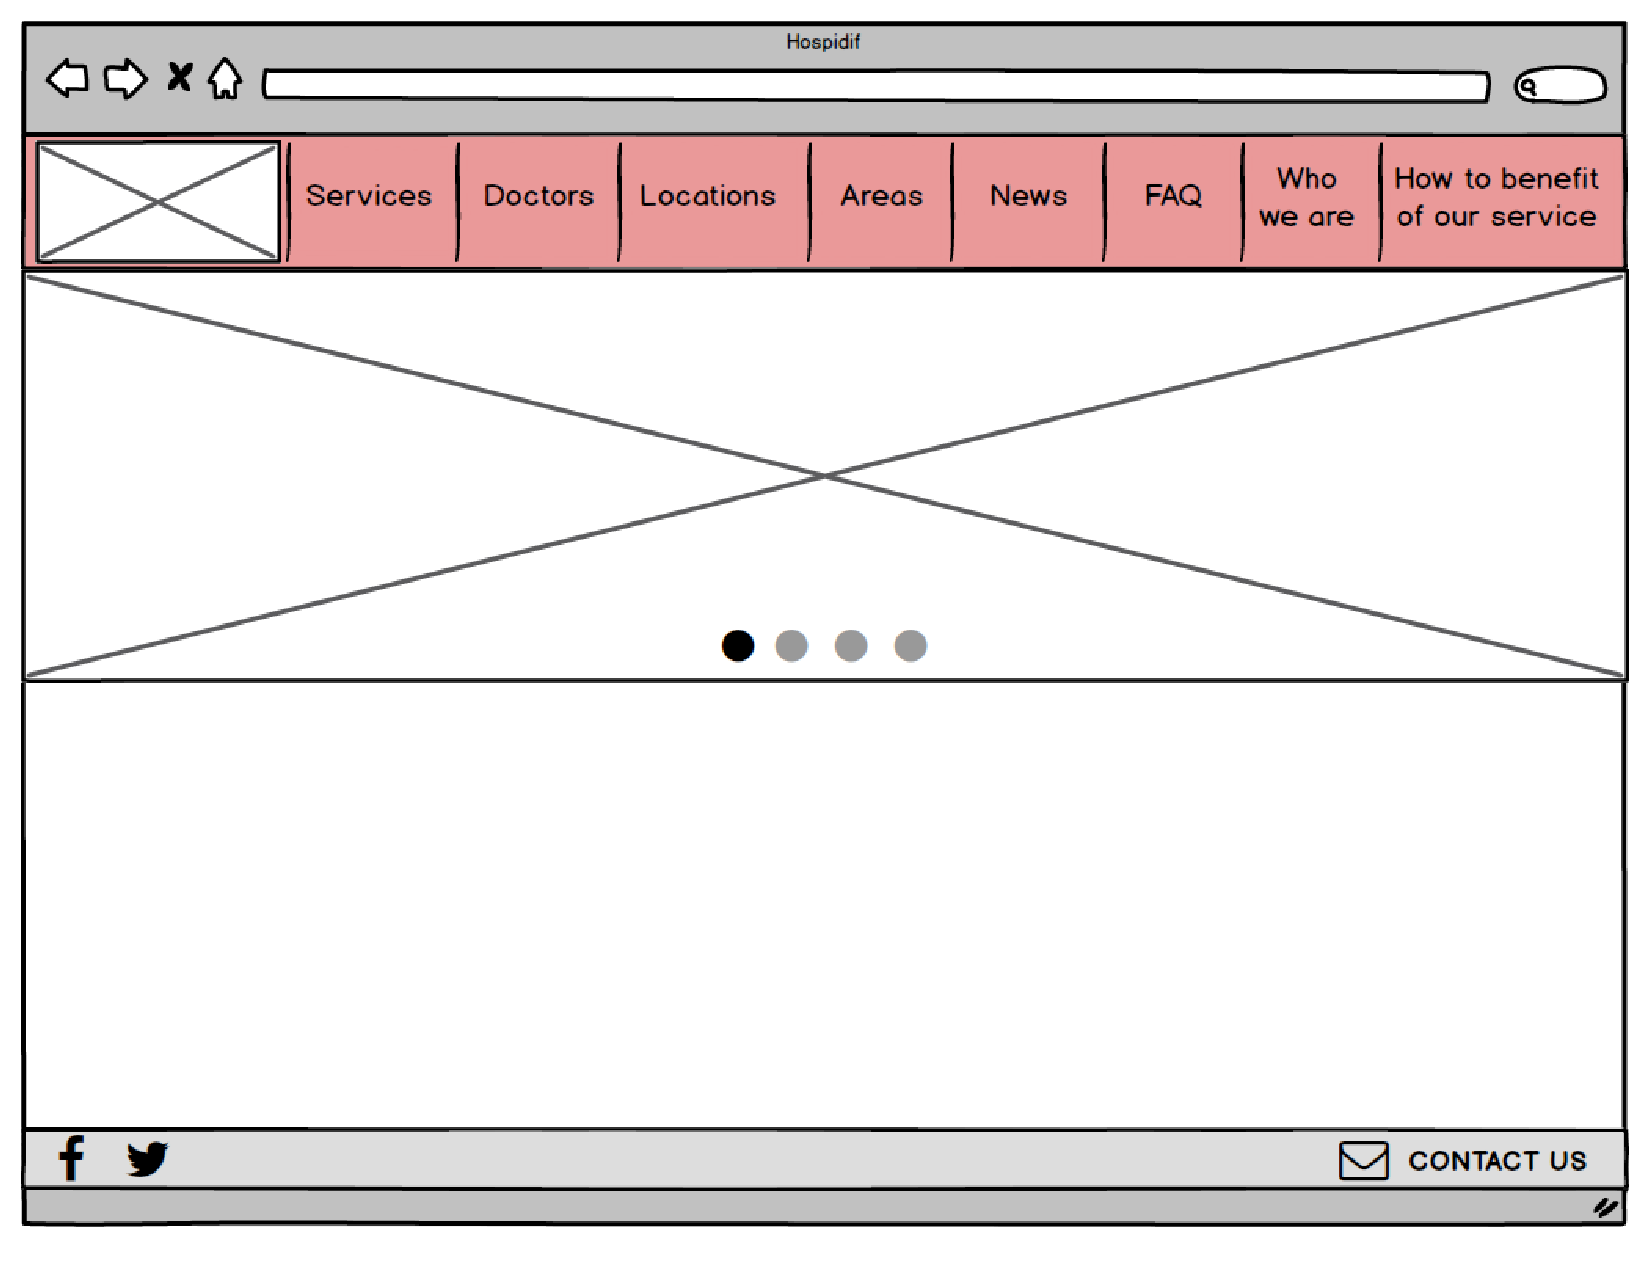
\includepdf[page=-,pagecommand={\pagestyle{fancy}}]{../Mockup/mockup.pdf}

\appendix
\chapter{Appendix}
\section{Version History}
In the following are listed the differences between versions:
\begin{itemize}
	\item 1.0.0: first release
\end{itemize}

\end{document}


